\documentclass[final,5p,times,twocolumn,authoryear]{elsarticle}
\usepackage[utf8]{inputenc}
\usepackage[T1]{fontenc}
\usepackage{graphicx}
\graphicspath{{./}{classification/}{eda/}{gradcam/}{pseudo_labeling_v2/}{segmentation_v1/}}
\usepackage{amsmath}
\usepackage[round,authoryear]{natbib}
\usepackage{url}
\usepackage{booktabs}
\usepackage{multirow}
\usepackage{xcolor}
\usepackage{tikz}
\usetikzlibrary{arrows.meta, positioning, fit, calc}
\usepackage{dblfloatfix}
\usepackage{adjustbox}
\usepackage[section]{placeins}

\setcounter{topnumber}{5}
\setcounter{bottomnumber}{5}
\setcounter{totalnumber}{8}
\setcounter{dbltopnumber}{5}
\renewcommand{\topfraction}{0.95}
\renewcommand{\bottomfraction}{0.9}
\renewcommand{\textfraction}{0.05}
\renewcommand{\floatpagefraction}{0.85}
\renewcommand{\dbltopfraction}{0.95}
\renewcommand{\dblfloatpagefraction}{0.85}

\definecolor{stageblue}{HTML}{DCEBFF}
\definecolor{stagegreen}{HTML}{DDF4E7}
\definecolor{stageorange}{HTML}{FFE8CC}
\definecolor{stagegray}{HTML}{EEF1F5}
\definecolor{stagepurple}{HTML}{EDE4FF}
\definecolor{arrowgray}{HTML}{4B5563}

\tikzset{
    pipelinebox/.style={
        draw=arrowgray,
        rounded corners=2pt,
        align=center,
        minimum width=3.1cm,
        minimum height=1.15cm,
        font=\small,
        inner sep=5pt
    },
    data/.style={pipelinebox, fill=stagegray},
    classmodel/.style={pipelinebox, fill=stageblue},
    xai/.style={pipelinebox, fill=stageorange},
    sam/.style={pipelinebox, fill=stagepurple},
    segmodel/.style={pipelinebox, fill=stagegreen},
    flow/.style={-{Latex[length=2.6mm]}, thick, draw=arrowgray},
    dashedflow/.style={-{Latex[length=2.6mm]}, thick, dashed, draw=arrowgray},
    lane/.style={draw=arrowgray!45, rounded corners=4pt, inner sep=8pt}
}

\begin{document}

\begin{frontmatter}

\journal{Data and Information Management}

\title{An explainable weakly supervised framework for durian leaf disease classification and lesion segmentation using EfficientNet and U-Net}

\author[aff1]{Van Lam Ho}
\author[aff2]{Minh Hieu Doan\corref{cor1}}
% TODO: Replace with the corresponding author's institutional email before submission.
% \ead{corresponding.author@institution.edu}
\author[aff3]{Nguyen Quynh Nhi Tran}

\cortext[cor1]{Corresponding author.}

\affiliation[aff1]{
    organization={Faculty of Information Technology, Quy Nhon University},
    city={Gia Lai},
    country={Vietnam}
}

\affiliation[aff2]{
    organization={Quy Nhon AI Research and Application Center, FPT Software},
    city={Gia Lai},
    country={Vietnam}
}

\affiliation[aff3]{
    organization={Faculty of Mathematics and Computer Science, Dalat University},
    city={Lam Dong},
    country={Vietnam}
}

\begin{abstract}
Accurate detection of durian (\textit{Durio zibethinus}) leaf disease is important for orchard management, but pixel-level lesion annotation remains costly and depends on expert judgement. This study develops a weakly supervised workflow that starts from image-level disease labels and produces both class predictions and lesion masks. An EfficientNet-B0 classifier first learns five durian leaf classes and reaches 97.52\% test accuracy. Multi-scale GradCAM++ maps are then converted into pseudo-masks for 3{,}104 training images by class-specific percentile thresholding. The masks are refined with the Segment Anything Model (SAM ViT-B) and used to train a UNet++ lesion segmentation model. When architecture, data split, and random seed are held fixed, SAM-refined labels improve IoU from 0.5135 to 0.6239 (+21.5\%) and Dice from 0.6301 to 0.7053 (+11.9\%). The experiments also show that segmentation scores from different pseudo-label sources should not be compared as absolute measures of disease localization. In particular, a one-sided IoU guard can accept SAM masks that expand from a lesion to a larger leaf region. These results support the use of classifier explanations as a practical source of weak spatial supervision, while also showing where such supervision needs careful checking.
\end{abstract}

\begin{keyword}
Durian leaf disease \sep Deep learning \sep EfficientNet \sep GradCAM++ \sep Pseudo-labeling \sep UNet++ \sep Segment Anything Model \sep Weakly supervised segmentation \sep Agricultural AI
\end{keyword}

\end{frontmatter}

\section{Introduction}

Durian (\textit{Durio zibethinus}) is one of the most economically significant tropical fruit crops in Southeast Asia, with Thailand, Malaysia, Indonesia, and Vietnam among the leading producers. Because fruit quality and yield are highly sensitive to foliar health, leaf diseases represent a persistent threat to grower income and to the sustainability of durian cultivation. Timely and accurate identification of disease symptoms is needed for targeted intervention, judicious use of agrochemicals, and crop management at plantation scale.

Conventional disease diagnosis relies on visual inspection by trained agronomists. This practice is labour-intensive, subjective, and difficult to scale to large orchards, and it typically identifies a problem only after symptoms have become severe. The maturation of deep learning and computer vision has motivated a large body of work on automated plant disease recognition, which now routinely achieves high classification accuracy across many crops \citep{mohanty2016using, ferentinos2018deep}. However, two gaps limit the practical value of most existing systems for durian. First, the majority of methods perform image-level classification only: they report \emph{whether} a leaf is diseased but not \emph{where} the lesions are, whereas spatial localization is what enables precise, site-specific treatment. Second, models that do produce pixel-level segmentation depend on dense manual annotation, which is costly, slow, and requires domain expertise that is rarely available for a specialty crop such as durian.

This work addresses three coupled challenges in durian leaf disease analysis:
\begin{enumerate}
\item \textbf{Annotation scarcity.} Pixel-level masks for plant lesions are expensive and expert-dependent; most accessible durian data carry only image-level labels.
\item \textbf{Interpretability.} Opaque deep models are difficult for agronomists to trust or validate, which impedes adoption in the field.
\item \textbf{Precise localization.} Classification alone cannot delineate the position and extent of lesions, information that is essential for targeted, resource-efficient treatment.
\end{enumerate}

To address these issues, we use an image-level classifier as the starting point for lesion segmentation. Class activation maps provide the initial spatial cues, and SAM is used only as a boundary refinement step. The main contributions are:
\begin{itemize}
\item A four-stage weakly supervised workflow linking classification, GradCAM++ pseudo-labeling, SAM refinement, and UNet++ segmentation using only image-level labels.
\item A multi-scale GradCAM++ pseudo-labeling method with \emph{per-class percentile thresholding}, designed to control mask coverage and reduce the over-segmentation observed with Otsu thresholding on smooth heatmaps.
\item An analysis of SAM ViT-B as a label refiner, including a failure case in which a one-sided Intersection-over-Union (IoU) guard does not reject masks that expand toward the whole leaf.
\item A comparison protocol that separates the V1/V2/V3 headline scores from the only matched comparison in the study, namely V2 to V3 under the same split, architecture, and seed.
\end{itemize}

The remainder of the paper is organised as follows. Section~\ref{sec:related} reviews related work on plant disease detection, explainable AI, weakly supervised segmentation, and segmentation foundation models. Section~\ref{sec:method} describes the dataset and the four stages of the method. Section~\ref{sec:results} reports and discusses the experimental results, including the comparability caveat and the SAM expansion analysis. Section~\ref{sec:conclusion} concludes and outlines future directions.

\section{Related work}
\label{sec:related}

\subsection{Deep learning for plant disease detection}

Convolutional neural networks (CNNs) have become the standard tool for image-based plant disease recognition, with successful applications across crops such as tomato, rice, and wheat \citep{mohanty2016using, ferentinos2018deep}. Because agricultural datasets are typically small relative to general-purpose vision corpora, transfer learning from ImageNet-pretrained backbones such as VGG, ResNet, and EfficientNet is common practice \citep{deng2009imagenet, tan2019efficientnet}. EfficientNet in particular offers a favourable accuracy-to-parameter trade-off through compound scaling of network depth, width, and input resolution \citep{tan2019efficientnet}, which makes it attractive for deployment-constrained agricultural settings. Most of these systems, however, stop at image-level classification and cannot indicate the spatial location or extent of the disease, limiting their usefulness for targeted treatment.

\subsection{Explainable AI in agricultural vision}

Interpretability matters in agricultural decision support because users need to know whether a model is responding to disease symptoms or to background cues. Gradient-weighted Class Activation Mapping (Grad-CAM) and related methods show which image regions influence a prediction \citep{selvaraju2017grad}. GradCAM++ improves localization for multiple and small objects by using second-order gradient information \citep{chattopadhay2018grad}, which is relevant for leaf diseases that often appear as scattered lesions. In this study, class activation maps are used not only for inspection but also as weak spatial supervision for segmentation.

\subsection{Weakly supervised segmentation and pseudo-labeling}

Weakly supervised segmentation aims to estimate pixel-level masks from cheaper labels such as image tags. Class activation maps are often used for this purpose because they provide coarse localization cues that can be thresholded and post-processed into pseudo-masks \citep{barbedo2019plant}. The main difficulty is that CAMs are low-resolution and often cover only the most discriminative part of an object. Pseudo-label quality depends heavily on thresholding and post-processing. In Section~\ref{sec:stage2v2}, we use multi-scale fusion together with per-class percentile thresholds as a practical alternative to Otsu thresholding, whose bimodality assumption is poorly matched to smooth fused heatmaps \citep{otsu1979threshold}.

\subsection{Segmentation foundation models}

The Segment Anything Model (SAM) is a promptable segmentation model trained on eleven million images and over one billion masks \citep{kirillov2023segment}. Given point, box, or mask prompts, SAM can produce sharp object boundaries and has been used in settings where manual annotation is limited. Here, SAM is not treated as a stand-alone disease segmenter. It is used as a refinement step for coarse GradCAM++ pseudo-masks, and its behaviour is checked for both boundary improvement and mask expansion. The segmentation networks used in the experiments build on U-Net \citep{ronneberger2015unet} and the nested UNet++ variant \citep{zhou2018unet++}.

\subsection{Positioning of this work}

Compared with previous work, this study focuses on a durian-specific setting with image-level labels only. It combines GradCAM++ pseudo-labeling with SAM refinement, uses class-aware coverage targets instead of a single unsupervised threshold, and reports which segmentation comparisons are matched and which are not. This distinction is important because pseudo-label-based scores can be misleading when each model is evaluated against labels produced by a different procedure.

\section{Materials and methods}
\label{sec:method}

\begin{figure*}[!t]
\centering
\resizebox{\textwidth}{!}{%
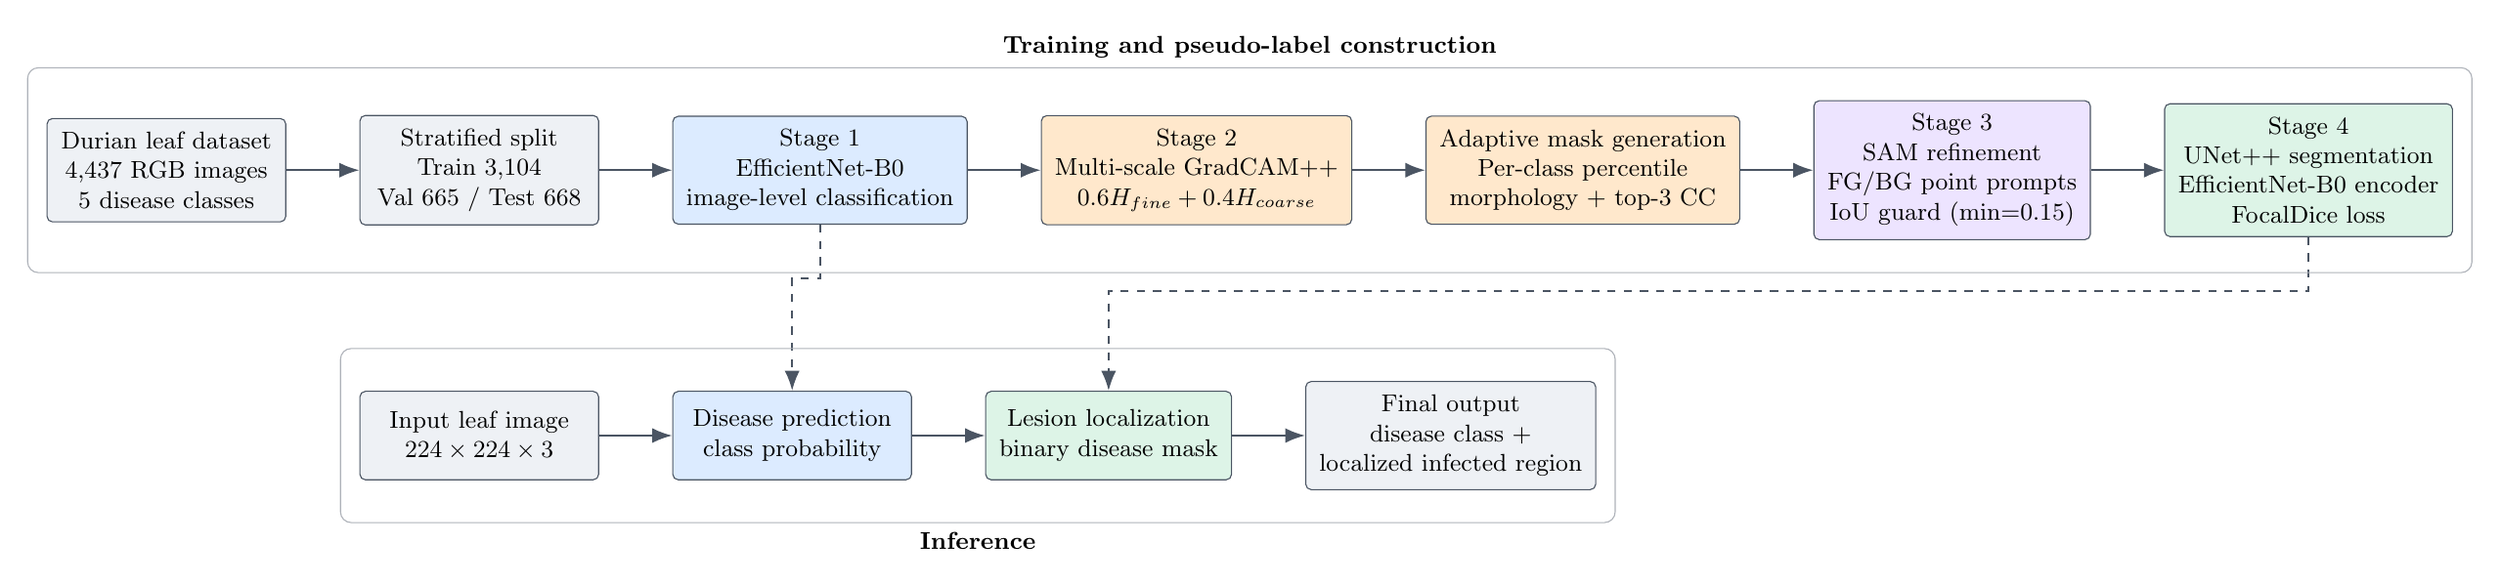
\begin{tikzpicture}[node distance=0.85cm and 0.95cm]
    \node[data] (dataset) {Durian leaf dataset\\4,437 RGB images\\5 disease classes};
    \node[data, right=of dataset] (split) {Stratified split\\Train 3,104\\Val 665 / Test 668};
    \node[classmodel, right=of split] (classifier) {Stage 1\\EfficientNet-B0\\image-level classification};
    \node[xai, right=of classifier] (gradcam) {Stage 2\\Multi-scale GradCAM++\\$0.6H_{fine}+0.4H_{coarse}$};
    \node[xai, right=of gradcam] (post) {Adaptive mask generation\\Per-class percentile\\morphology + top-3 CC};
    \node[sam, right=of post] (samrefine) {Stage 3\\SAM refinement\\FG/BG point prompts\\IoU guard (min=0.15)};
    \node[segmodel, right=of samrefine] (segtrain) {Stage 4\\UNet++ segmentation\\EfficientNet-B0 encoder\\FocalDice loss};

    \node[data, below=2.15cm of split] (newimage) {Input leaf image\\$224\times224\times3$};
    \node[classmodel, right=of newimage] (inferclass) {Disease prediction\\class probability};
    \node[segmodel, right=of inferclass] (inferseg) {Lesion localization\\binary disease mask};
    \node[data, right=of inferseg] (decision) {Final output\\disease class +\\localized infected region};

    \draw[flow] (dataset) -- (split);
    \draw[flow] (split) -- (classifier);
    \draw[flow] (classifier) -- (gradcam);
    \draw[flow] (gradcam) -- (post);
    \draw[flow] (post) -- (samrefine);
    \draw[flow] (samrefine) -- (segtrain);

    \draw[dashedflow] (classifier.south) -- ++(0,-0.7) -| (inferclass.north);
    \draw[dashedflow] (segtrain.south) -- ++(0,-0.7) -| (inferseg.north);
    \draw[flow] (newimage) -- (inferclass);
    \draw[flow] (inferclass) -- (inferseg);
    \draw[flow] (inferseg) -- (decision);

    \node[lane, fit=(dataset)(split)(classifier)(gradcam)(post)(samrefine)(segtrain), inner xsep=7pt, inner ysep=12pt,
        label={[font=\bfseries\small]above:Training and pseudo-label construction}] {};
    \node[lane, fit=(newimage)(inferclass)(inferseg)(decision), inner xsep=7pt, inner ysep=12pt,
        label={[font=\bfseries\small]below:Inference}] {};
\end{tikzpicture}%
}
\caption{Overview of the proposed weakly supervised durian leaf disease analysis workflow. The classification model learns image-level disease categories, after which multi-scale GradCAM++ maps are converted into pseudo-segmentation masks using per-class percentile thresholding. SAM refines these masks before they are used to train the final UNet++ lesion-segmentation model. At inference time, the system returns both the disease class and the localized infected region.}
\label{fig:proposed_pipeline}
\end{figure*}

\subsection{Dataset}

The dataset comprises 4{,}437 durian leaf images collected from plantations in Southeast Asia, organised into five classes: Algal Leaf Spot (733 images), Allocaridara Attack (913 images), Healthy Leaf (976 images), Leaf Blight (937 images), and Phomopsis Leaf Spot (878 images).

\begin{figure*}[!t]
\centering
\includegraphics[width=\textwidth]{eda/sample_images_per_class.png}
\caption{Representative samples from the five durian leaf classes used in the experiments, illustrating the visual diversity of healthy leaves and disease symptoms under field imaging conditions.}
\label{fig:dataset_samples}
\end{figure*}

The data were partitioned into training (70\%, 3{,}104 images), validation (15\%, 665 images), and test (15\%, 668 images) sets by stratified sampling to preserve the class distribution. For the segmentation stages (Stages~2--4), the same 3{,}104 training images were used for pseudo-label generation and then re-split 70/15/15 (2{,}172 train / 465 validation / 467 test) with a fixed seed (42) to ensure reproducibility and a consistent evaluation basis across workflow versions.

\subsection{Stage 1: Image-level classification}

\subsubsection{Architecture}

We adopt EfficientNet-B0 as the classification backbone for its favourable balance between accuracy and computational cost \citep{tan2019efficientnet}. The network takes $224\times224\times3$ RGB inputs, applies an ImageNet-pretrained EfficientNet-B0 backbone \citep{deng2009imagenet}, global average pooling, a fully connected layer with five outputs, and a softmax activation.

\subsubsection{Training configuration}

The classifier was optimised with Adam (learning rate $1\times10^{-4}$) under a cross-entropy objective, a batch size of 32, and up to 30 epochs with learning-rate reduction on plateau (ReduceLROnPlateau, patience~=~2, factor~=~0.5). Data augmentation comprised random horizontal and vertical flips, rotation, and colour jitter.

\subsubsection{Results}

The model reached 97.52\% test accuracy with a mean inference confidence of 0.9822 across the 3{,}104 training images subsequently used for pseudo-label generation. Consistently high-confidence predictions are important because they yield reliable class activation maps to serve as segmentation seeds in Stage~2.

\subsection{Stage 2 (baseline, V1): single-scale GradCAM pseudo-labels}

As a baseline, single-layer Grad-CAM was applied to the final convolutional layer (\texttt{features.8}, $7\times7$ resolution) with a fixed threshold of 0.5 and a rectangular $5\times5$ morphological kernel, on a 500-image subset (100 per class). This configuration defines the segmentation baseline referred to as V1 in Section~\ref{sec:seg_results}.

\subsection{Stage 2 (improved, V2): multi-scale GradCAM++ with per-class percentile thresholding}
\label{sec:stage2v2}

\subsubsection{Multi-scale GradCAM++}

Single-scale Grad-CAM often fails to capture multiple small lesions because of spatial averaging. We combine GradCAM++ activations from two resolution levels. Fine-grained features ($14\times14$, \texttt{features.6}) improve the localization of small lesions and preserve spot detail, whereas coarse features ($7\times7$, \texttt{features.8}) provide semantic context and suppress background false positives. The fused heatmap is
\begin{equation}
H_{final} = 0.6 \times H_{fine} + 0.4 \times H_{coarse}.
\end{equation}
GradCAM++ refines standard Grad-CAM by weighting activations with second-order gradient information \citep{chattopadhay2018grad}:
\begin{equation}
\alpha_k^c = \frac{\frac{\partial^2 y^c}{\partial A_k^2}}{2\frac{\partial^2 y^c}{\partial A_k^2} + \sum A_k \frac{\partial^3 y^c}{\partial A_k^3}},
\end{equation}
\begin{equation}
w_k^c = \sum \alpha_k^c \times \text{ReLU}\left(\frac{\partial y^c}{\partial A_k}\right),
\end{equation}
where $A_k$ denotes activation maps and $y^c$ the class score.

\subsubsection{Per-class percentile thresholding}

Rather than Otsu's method \citep{otsu1979threshold}, which assumes a bimodal heatmap distribution and over-segments when multi-scale fusion produces smooth gradients, we apply a per-class percentile threshold that directly controls mask coverage (Table~\ref{tab:percentile}).

\begin{table}[!htbp]
\centering
\caption{Per-class coverage targets for percentile thresholding.}
\label{tab:percentile}
\begin{adjustbox}{max width=\columnwidth}
\begin{tabular}{lcc}
\toprule
\textbf{Class} & \textbf{Keep top \%} & \textbf{Rationale} \\
\midrule
Algal Leaf Spot     & 18\% & Compact spot lesions \\
Allocaridara Attack & 20\% & Moderate-area insect damage \\
Healthy Leaf        & 0\%  & No lesion tissue \\
Leaf Blight         & 22\% & Diffuse blight patches \\
Phomopsis Leaf Spot & 18\% & Compact spot lesions \\
\bottomrule
\end{tabular}
\end{adjustbox}
\end{table}

The threshold is the $(1-p)\times100^{\text{th}}$ percentile of each heatmap, where $p$ is the target coverage fraction. Assigning Healthy Leaf an all-zero mask removes the $\sim$683 false-positive masks that would otherwise be generated for disease-free images. The trade-off is that coverage is fixed per class and does not adapt to disease severity in each image.

\subsubsection{Post-processing}

Two post-processing steps clean the thresholded masks: (i) morphological closing followed by opening with a $5\times5$ elliptical kernel to fill holes and remove noise, and (ii) connected-component filtering that retains the top three components of at least 400 pixels, removing mid-size noise fragments while preserving multiple lesion spots. This procedure produced 3{,}104 pseudo-labeled masks from the full training set.

\begin{figure*}[!t]
\centering
\includegraphics[width=\textwidth]{gradcam/gradcam_samples_per_class_landscape.png}
\caption{GradCAM++ activation maps for representative samples from each disease class. The heatmaps mark the regions used by the classifier and are later thresholded to generate pseudo-segmentation masks.}
\label{fig:gradcam_samples}
\end{figure*}

\begin{figure*}[!t]
\centering
\includegraphics[width=\textwidth]{pseudo_labeling_v2/v1_vs_v2_comparison.png}
\caption{Pseudo-label quality: single-scale Grad-CAM V1 (fixed threshold 0.5) versus multi-scale GradCAM++ with per-class percentile thresholding (V2). The V2 approach produces coverage-controlled, cleaner masks, with noise fragments removed by top-3 connected-component filtering.}
\label{fig:pseudolabel_comparison}
\end{figure*}

\subsection{Stage 3: SAM boundary refinement}

\subsubsection{Motivation and prompt generation}

GradCAM++ localises lesions well but yields blurry boundaries because of the low resolution of the activation maps ($7\times7$ or $14\times14$). SAM excels at pixel-accurate boundary delineation given suitable prompts \citep{kirillov2023segment}. For each V2 pseudo-mask we extract foreground prompts (the mask centroid plus five points sampled from the masked region) and background prompts (three points sampled from the dilated complement, using a 30-pixel dilation) so that SAM can distinguish diseased from healthy tissue.

\subsubsection{IoU guard and fallback}

To prevent SAM from drifting to an incorrect region, we apply an IoU guard between the SAM output and the GradCAM++ mask:
\begin{equation}
\text{IoU} = \frac{|\text{SAM}_{mask} \cap \text{GradCAM}_{mask}|}{|\text{SAM}_{mask} \cup \text{GradCAM}_{mask}|},
\end{equation}
\begin{equation}
\text{refined}_{mask} = \begin{cases}
\text{SAM}_{mask} & \text{if IoU} \geq 0.15, \\
\text{GradCAM}_{mask} & \text{otherwise.}
\end{cases}
\end{equation}

\subsubsection{Coverage expansion: a failure mode of the one-sided guard}

SAM often expands masks beyond the intended lesion area (Table~\ref{tab:sam_expansion}). With point prompts, the model tends to segment a larger semantic unit, often much of the leaf, rather than only the lesion.

\begin{table}[!htbp]
\centering
\caption{Coverage expansion from V2 pseudo-labels to SAM-refined labels.}
\label{tab:sam_expansion}
\begin{adjustbox}{max width=\columnwidth}
\begin{tabular}{lccc}
\toprule
\textbf{Class} & \textbf{V2 coverage} & \textbf{SAM coverage} & \textbf{$\Delta$} \\
\midrule
Algal Leaf Spot     & 17.7\% & 35.0\% & +97\% \\
Allocaridara Attack & 19.7\% & 32.0\% & +62\% \\
Leaf Blight         & 21.7\% & 30.7\% & +41\% \\
Phomopsis Leaf Spot & 17.6\% & 33.6\% & +91\% \\
\midrule
\textbf{Overall}    & \textbf{15.0\%} & \textbf{25.5\%} & \textbf{+70\%} \\
\bottomrule
\end{tabular}
\end{adjustbox}
\end{table}

In total, 211 of 3{,}104 masks (6.8\%) exceeded 50\% coverage after refinement. The guard does not catch this expansion. When SAM segments the whole leaf and the V2 lesion is fully contained within it, the IoU equals the V2 coverage divided by the SAM coverage ($\approx0.51 > 0.15$). The guard triggers only when SAM \emph{drifts} to a disjoint region, not when it \emph{expands} to contain the original mask. A two-sided coverage-ratio constraint, for example falling back to the V2 mask if $\text{SAM coverage} > 2\times\text{V2 coverage}$, would address this limitation.

\subsection{Stage 4: Lesion segmentation}

\subsubsection{Architecture}

The baseline V1 uses a custom EfficientNet-U-Net trained with a combined BCE and Dice loss (Adam with ReduceLROnPlateau, 30 epochs). The improved V2 and V3 configurations use UNet++ \citep{zhou2018unet++} with an ImageNet-pretrained EfficientNet-B0 encoder, nested dense skip connections in the decoder, and a single-channel binary output (disease versus background); the model has 6{,}569{,}581 trainable parameters. The dense skip connections of UNet++ reduce the semantic gap between encoder and decoder and improve small-object segmentation relative to plain U-Net \citep{ronneberger2015unet}.

\subsubsection{Training configuration (V2/V3)}

The segmentation objective is a FocalDice loss:
\begin{equation}
\mathcal{L}_{total} = \mathcal{L}_{focal} + \mathcal{L}_{dice},
\end{equation}
\begin{equation}
\mathcal{L}_{focal} = -\alpha(1-p_t)^\gamma \log(p_t), \quad \alpha=0.25,\ \gamma=2.0,
\end{equation}
\begin{equation}
\mathcal{L}_{dice} = 1 - \frac{2|X \cap Y| + \epsilon}{|X| + |Y| + \epsilon},
\end{equation}
where the focal term follows \citet{lin2017focal}. Optimisation used AdamW \citep{loshchilov2019decoupled} (learning rate $1\times10^{-4}$, weight decay $1\times10^{-4}$), a CosineAnnealingLR schedule ($T_{max}=50$, $\eta_{min}=1\times10^{-6}$), a batch size of 4, up to 50 epochs with early stopping on validation loss (patience~=~10), and gradient clipping at a maximum norm of 1.0. Augmentation comprised RandomResizedCrop, horizontal/vertical flips, RandomRotate90, ShiftScaleRotate, ElasticTransform, GridDistortion, ColorJitter, and GaussNoise \citep{buslaev2020albumentations}.

\section{Results and discussion}
\label{sec:results}

\subsection{Classification performance}

EfficientNet-B0 achieved high test performance across all five classes (Table~\ref{tab:classification}), with similar per-class scores (Table~\ref{tab:classification_perclass}).

\begin{table}[!htbp]
\centering
\caption{Classification performance on the test set.}
\label{tab:classification}
\begin{adjustbox}{max width=\columnwidth}
\begin{tabular}{lcc}
\toprule
\textbf{Metric} & \textbf{Best validation} & \textbf{Test} \\
\midrule
Accuracy  & 97.52\% & 97.52\% \\
Precision & N/A     & 97.34\% \\
Recall    & N/A     & 97.30\% \\
F1-score  & N/A     & 97.31\% \\
\bottomrule
\end{tabular}
\end{adjustbox}
\end{table}

\begin{table}[!htbp]
\centering
\caption{Per-class classification performance on the test set.}
\label{tab:classification_perclass}
\begin{adjustbox}{max width=\columnwidth}
\begin{tabular}{lcccc}
\toprule
\textbf{Class} & \textbf{Precision} & \textbf{Recall} & \textbf{F1} & \textbf{Samples} \\
\midrule
Algal Leaf Spot     & 94.70\% & 97.28\% & 95.97\% & 147 \\
Allocaridara Attack & 98.90\% & 98.36\% & 98.63\% & 183 \\
Healthy Leaf        & 96.95\% & 97.45\% & 97.20\% & 196 \\
Leaf Blight         & 100.00\% & 96.28\% & 98.10\% & 188 \\
Phomopsis Leaf Spot & 95.53\% & 97.16\% & 96.34\% & 176 \\
\midrule
\textbf{Weighted avg.} & \textbf{97.34\%} & \textbf{97.30\%} & \textbf{97.31\%} & \textbf{890} \\
\bottomrule
\end{tabular}
\end{adjustbox}
\end{table}

\begin{figure*}[!t]
\centering
\includegraphics[width=\textwidth]{classification/training_curves.png}
\caption{Training and validation curves for the EfficientNet-B0 classifier. A test accuracy of 97.52\% is achieved with balanced per-class F1 scores of 0.96--0.99.}
\label{fig:classification_training_curves}
\end{figure*}

\begin{figure}[!htbp]
\centering
\includegraphics[width=\columnwidth]{classification/confusion_matrix.png}
\caption{Confusion matrix on the test set. Most misclassifications occur between visually similar classes, particularly Algal Leaf Spot and Phomopsis Leaf Spot.}
\label{fig:confusion_matrix}
\end{figure}

\subsection{Pseudo-label quality}

The V2 coverage targets were met with less than 0.4\% deviation per class (Table~\ref{tab:v2_coverage}). Setting Healthy Leaf coverage to zero removes the $\sim$683 false-positive masks that would otherwise arise for a disease-free class.

\begin{table}[!htbp]
\centering
\caption{V2 pseudo-label coverage statistics.}
\label{tab:v2_coverage}
\begin{adjustbox}{max width=\columnwidth}
\begin{tabular}{lccc}
\toprule
\textbf{Class} & \textbf{Actual coverage} & \textbf{Std} & \textbf{Target} \\
\midrule
Algal Leaf Spot     & 17.7\% & 0.008 & 18\% \\
Allocaridara Attack & 19.7\% & 0.007 & 20\% \\
Healthy Leaf        & 0.0\%  & 0.000 & 0\%  \\
Leaf Blight         & 21.7\% & 0.007 & 22\% \\
Phomopsis Leaf Spot & 17.6\% & 0.009 & 18\% \\
\bottomrule
\end{tabular}
\end{adjustbox}
\end{table}

\subsection{Segmentation performance}
\label{sec:seg_results}

Three segmentation configurations were evaluated (Table~\ref{tab:segmentation}). V1 differs from V2/V3 in dataset subset, architecture, and pseudo-label distribution, so its score should not be read as a direct comparison; Section~\ref{sec:caveat} discusses this constraint.

\begin{table}[!htbp]
\centering
\caption{Segmentation performance on the test set.}
\label{tab:segmentation}
\footnotesize
\begin{adjustbox}{max width=\columnwidth}
\begin{tabular}{lccccc}
\toprule
\textbf{Version} & \textbf{IoU} & \textbf{Dice} & \textbf{Precision} & \textbf{Recall} & \textbf{F1} \\
\midrule
V1$^\dagger$ & 0.7671 & 0.8623 & 0.8562 & 0.8877 & 0.8623 \\
V2           & 0.5135 & 0.6301 & 0.6169 & 0.7419 & 0.6301 \\
V3           & \textbf{0.6239} & \textbf{0.7053} & \textbf{0.7090} & \textbf{0.8752} & \textbf{0.7053} \\
\bottomrule
\end{tabular}
\end{adjustbox}
\par\smallskip
\raggedright\scriptsize V1: EfficientNet-U-Net with Grad-CAM V1 labels. V2: UNet++ with GradCAM++ percentile labels. V3: UNet++ with SAM-refined labels. $^\dagger$ V1 uses a different dataset subset, architecture, and label distribution from V2/V3, so it is not directly comparable.
\end{table}

The matched comparison is V2~$\to$~V3, where architecture, split, and seed are held constant (Table~\ref{tab:v2v3}).

\begin{table}[!htbp]
\centering
\caption{V2 versus V3 segmentation improvement (same architecture, split, and seed).}
\label{tab:v2v3}
\begin{adjustbox}{max width=\columnwidth}
\begin{tabular}{lccc}
\toprule
\textbf{Metric} & \textbf{V2} & \textbf{V3} & \textbf{$\Delta$} \\
\midrule
IoU       & 0.5135 & 0.6239 & \textbf{+21.5\%} \\
Dice      & 0.6301 & 0.7053 & +11.9\% \\
Precision & 0.6169 & 0.7090 & +14.9\% \\
Recall    & 0.7419 & 0.8752 & +18.0\% \\
\bottomrule
\end{tabular}
\end{adjustbox}
\end{table}

In this matched setting, SAM boundary refinement improves all reported metrics, suggesting that sharper training targets are easier for UNet++ to learn than the coarse GradCAM++ masks.

\begin{figure*}[!t]
\centering
\includegraphics[width=0.92\textwidth]{segmentation_v1/training_curves.png}
\caption{Training and validation curves for the V1 segmentation model (EfficientNet-U-Net, 30 epochs), reaching a best validation IoU of 0.7715 and Dice of 0.8650.}
\label{fig:seg_v1_curves}
\end{figure*}

\begin{figure*}[!t]
\centering
\includegraphics[width=0.66\textwidth,height=0.72\textheight,keepaspectratio]{segmentation_v1/test_predictions.png}
\caption{V1 segmentation test predictions showing the input image, pseudo-label reference, predicted probability map, and binary prediction with IoU/Dice scores.}
\label{fig:seg_v1_predictions}
\end{figure*}

\subsection{Cross-version comparability caveat}
\label{sec:caveat}

The V1 versus V2/V3 comparison must be interpreted with care because each version is evaluated against \emph{its own pseudo-labels}. V1 (IoU~=~0.767) learns simple Grad-CAM blobs generated by a fixed threshold of 0.5. These masks are relatively smooth and easy to reproduce. V3 (IoU~=~0.624) learns SAM-shaped boundaries that are sharper, more varied, and often larger. The higher IoU of V1 does \emph{not} imply better disease localization; it mainly reflects an easier reference mask. Without ground-truth pixel annotation, absolute localization accuracy cannot be established. For this reason, the matched V2~$\to$~V3 comparison is the most informative result in this study, showing a +21.5\% IoU gain after SAM boundary refinement.

\subsection{Training dynamics}

For V3 (22 epochs, early-stopped at epoch~22), validation loss and validation IoU were not monotonically aligned (Table~\ref{tab:v3_dynamics}). Early stopping on validation loss selected epoch~12 rather than epoch~17, with a gap of 0.050 IoU. The reported test IoU of 0.6239 corresponds to the epoch-12 checkpoint; selection by validation IoU would have produced a higher upper bound. V3 also converged faster than V2 (validation loss 0.4478 at epoch~12 versus 0.5957 at epoch~20), consistent with SAM labels providing a cleaner training signal.

\begin{table}[!htbp]
\centering
\caption{V3 key training checkpoints.}
\label{tab:v3_dynamics}
\begin{adjustbox}{max width=\columnwidth}
\begin{tabular}{lccc}
\toprule
\textbf{Checkpoint} & \textbf{Epoch} & \textbf{Validation loss} & \textbf{Validation IoU} \\
\midrule
Best loss (selected) & E12 & \textbf{0.4478} & 0.6479 \\
Best IoU (missed)    & E17 & 0.4537           & \textbf{0.6981} \\
\bottomrule
\end{tabular}
\end{adjustbox}
\end{table}

\subsection{Qualitative observations}

Across all versions, recall exceeds precision (V3: 0.875 versus 0.709), indicating a systematic tendency to over-segment that is inherited from the over-coverage of the pseudo-labels. The Healthy Leaf hard-zero masking eliminates false-positive lesion activations for disease-free images. Finally, the sharper boundaries supplied by SAM labels help UNet++ learn precise edge features, visible as a concentration of probability mass around lesion margins.

\subsection{Computational efficiency}

Training required approximately two hours for classification (16 epochs), about seven minutes for GradCAM++ pseudo-label generation and about 40 minutes for SAM refinement over 3{,}104 images, about three hours for V2 segmentation (25 epochs with early stopping), and about 2.5 hours for V3 segmentation (22 epochs with early stopping). At inference, a single image requires 15~ms for classification and 45~ms for segmentation, for a total of 60~ms, corresponding to real-time throughput of roughly 16~frames per second.

\subsection{Limitations}
\label{sec:limitations}

Several limitations remain. First, no ground-truth pixel annotation is available, so absolute segmentation accuracy cannot be established and cross-version comparisons are constrained as described in Section~\ref{sec:caveat}. Second, per-class percentile thresholding fixes coverage within each class and cannot adapt to severity in individual images. Third, the one-sided IoU guard does not prevent SAM mask expansion, which increases coverage by 41--97\% per class. Fourth, checkpoint selection based on validation loss can miss the validation-IoU optimum.

\FloatBarrier
\section{Conclusion}
\label{sec:conclusion}

This paper presented a weakly supervised approach for durian leaf disease analysis using only image-level labels. EfficientNet-B0 achieved 97.52\% test accuracy across five classes and produced class activation maps for pseudo-mask generation. The proposed percentile thresholds kept disease-class coverage within 18--22\%, assigned zero coverage to Healthy Leaf, and met the target values within 0.4\% deviation. In the matched V2~$\to$~V3 comparison, SAM boundary refinement improved IoU by +21.5\%. At the same time, SAM increased mask coverage by 41--97\% per class, showing that point-prompt refinement can expand from lesions to larger leaf regions. The results also show that pseudo-label-based segmentation scores should be interpreted with caution when no ground-truth masks are available, and that checkpoint selection by validation loss can miss the validation-IoU optimum by 0.050 IoU.

Future work will pursue five directions: (i) constructing a small manually annotated test set (50--100 images) to enable absolute performance validation and fair cross-version comparison; (ii) replacing the one-sided IoU guard with a two-sided coverage-ratio constraint to suppress mask expansion; (iii) selecting checkpoints on validation IoU rather than validation loss; (iv) integrating SAM2 for improved boundary accuracy and reduced coverage expansion; and (v) extending binary lesion segmentation to per-class multi-class segmentation and edge-device deployment via quantisation and pruning.

\section*{CRediT authorship contribution statement}
\noindent\textbf{Van Lam Ho:} Conceptualization, Methodology, Software, Validation, Formal analysis, Investigation, Writing -- original draft, Writing -- review \& editing. \textbf{Minh Hieu Doan:} Methodology, Software, Data curation, Validation, Writing -- review \& editing. \textbf{Nguyen Quynh Nhi Tran:} Investigation, Visualization, Data curation, Writing -- review \& editing.

\section*{Ethics approval and consent to participate}
\noindent This study used plant leaf images and did not involve human participants, human data, or animals.

\section*{Funding}
\noindent This research did not receive any specific grant from funding agencies in the public, commercial, or not-for-profit sectors.

\section*{Declaration of competing interest}
\noindent The authors declare that they have no known competing financial interests or personal relationships that could have appeared to influence the work reported in this paper.

\section*{Data availability}
\noindent The image data and trained model checkpoints are not publicly released with this manuscript because they contain project-specific research assets. Derived experiment summaries and reproducibility metadata are available in the accompanying project repository.

\section*{Acknowledgements}
\noindent The authors thank the research and technical collaborators who supported dataset preparation, model training, and manuscript review.

\begin{thebibliography}{99}

\bibitem[Barbedo(2019)]{barbedo2019plant}
Barbedo, J. G. A. (2019). Plant disease identification from individual lesions and spots using deep learning. \textit{Biosystems Engineering, 180}, 96--107.

\bibitem[Buslaev et al.(2020)]{buslaev2020albumentations}
Buslaev, A., Iglovikov, V. I., Khvedchenya, E., Parinov, A., Druzhinin, M., \& Kalinin, A. A. (2020). Albumentations: Fast and flexible image augmentations. \textit{Information, 11}(2), 125.

\bibitem[Chattopadhyay et al.(2018)]{chattopadhay2018grad}
Chattopadhyay, A., Sarkar, A., Howlader, P., \& Balasubramanian, V. N. (2018). Grad-CAM++: Generalized gradient-based visual explanations for deep convolutional networks. In \textit{Proceedings of the IEEE Winter Conference on Applications of Computer Vision (WACV)} (pp. 839--847).

\bibitem[Deng et al.(2009)]{deng2009imagenet}
Deng, J., Dong, W., Socher, R., Li, L.-J., Li, K., \& Fei-Fei, L. (2009). ImageNet: A large-scale hierarchical image database. In \textit{Proceedings of the IEEE Conference on Computer Vision and Pattern Recognition (CVPR)} (pp. 248--255).

\bibitem[Ferentinos(2018)]{ferentinos2018deep}
Ferentinos, K. P. (2018). Deep learning models for plant disease detection and diagnosis. \textit{Computers and Electronics in Agriculture, 145}, 311--318.

\bibitem[Kirillov et al.(2023)]{kirillov2023segment}
Kirillov, A., Mintun, E., Ravi, N., Mao, H., Rolland, C., Gustafson, L., et al. (2023). Segment anything. In \textit{Proceedings of the IEEE International Conference on Computer Vision (ICCV)} (pp. 4015--4026).

\bibitem[Lin et al.(2017)]{lin2017focal}
Lin, T.-Y., Goyal, P., Girshick, R., He, K., \& Doll\'{a}r, P. (2017). Focal loss for dense object detection. In \textit{Proceedings of the IEEE International Conference on Computer Vision (ICCV)} (pp. 2980--2988).

\bibitem[Loshchilov \& Hutter(2019)]{loshchilov2019decoupled}
Loshchilov, I., \& Hutter, F. (2019). Decoupled weight decay regularization. In \textit{Proceedings of the International Conference on Learning Representations (ICLR)}.

\bibitem[Mohanty et al.(2016)]{mohanty2016using}
Mohanty, S. P., Hughes, D. P., \& Salath\'{e}, M. (2016). Using deep learning for image-based plant disease detection. \textit{Frontiers in Plant Science, 7}, 1419.

\bibitem[Otsu(1979)]{otsu1979threshold}
Otsu, N. (1979). A threshold selection method from gray-level histograms. \textit{IEEE Transactions on Systems, Man, and Cybernetics, 9}(1), 62--66.

\bibitem[Ronneberger et al.(2015)]{ronneberger2015unet}
Ronneberger, O., Fischer, P., \& Brox, T. (2015). U-Net: Convolutional networks for biomedical image segmentation. In \textit{Proceedings of the International Conference on Medical Image Computing and Computer-Assisted Intervention (MICCAI)} (pp. 234--241).

\bibitem[Selvaraju et al.(2017)]{selvaraju2017grad}
Selvaraju, R. R., Cogswell, M., Das, A., Vedantam, R., Parikh, D., \& Batra, D. (2017). Grad-CAM: Visual explanations from deep networks via gradient-based localization. In \textit{Proceedings of the IEEE International Conference on Computer Vision (ICCV)} (pp. 618--626).

\bibitem[Tan \& Le(2019)]{tan2019efficientnet}
Tan, M., \& Le, Q. V. (2019). EfficientNet: Rethinking model scaling for convolutional neural networks. In \textit{Proceedings of the International Conference on Machine Learning (ICML)} (pp. 6105--6114).

\bibitem[Zhou et al.(2018)]{zhou2018unet++}
Zhou, Z., Siddiquee, M. M. R., Tajbakhsh, N., \& Liang, J. (2018). UNet++: A nested U-Net architecture for medical image segmentation. In \textit{Deep Learning in Medical Image Analysis and Multimodal Learning for Clinical Decision Support} (pp. 3--11).

\end{thebibliography}

\end{document}
